\subsubsection{Kräfte}

\begin{itemize}
	\item Die Haft und Gleitreibung ist unabhängig von der Fläche
	\item Bei der schrägen Ebene wählt man das  Koordinaten-System mit Vorteil parallel zur Gleitebene
	\item Körper von 1kg mit $1\frac{m}{s^2}$ beschleunigen = Es wirkt eine Kraft von $1N$
	\item Beschleunigungskraft in der Schiefen Ebene: $F_B = F_H - F_G$
\end{itemize}

\begin{minipage}[h!]{0.3\linewidth}
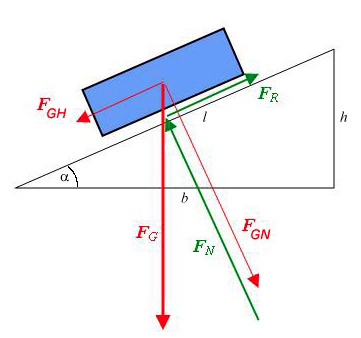
\includegraphics[width=0.9\linewidth]{images/schiefe_ebene}
\end{minipage}
\hfill
\begin{minipage}[h!]{0.2\linewidth}
	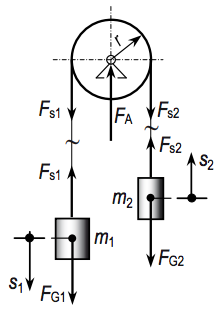
\includegraphics[width=0.9\linewidth]{images/kraefte_gleichgewicht}
\end{minipage}
\hfill
\begin{minipage}[h!]{0.4\linewidth}
\begin{align*}
m_1 \cdot a & = F_{G1} - F_{s1} \\
m_2 \cdot a & = -F_{G2} + F_{s2} \\
\Rightarrow a&=g\frac{m_1-m_2}{m_1+m_2}  \\
\Rightarrow \alpha &= \frac{a}{r} (\text{Winkelgeschwindigkeit})\\
\end{align*}
\end{minipage}

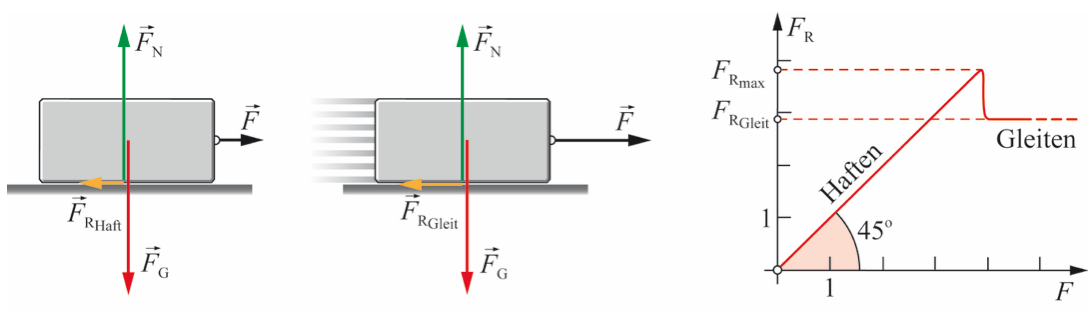
\includegraphics[width=0.9\linewidth]{images/haft_gleitkraft}


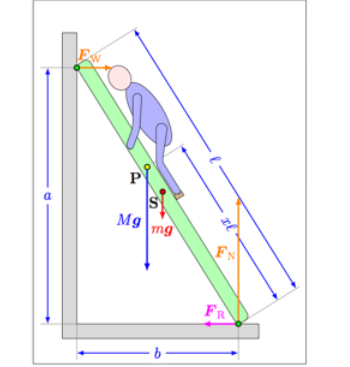
\includegraphics[width=0.3\linewidth]{images/leiter_kraefte}


\begin{tabbing}
	\begin{tabu} to \linewidth {X l X l}
		\toprule
		Kraft & $F = m \cdot a$ & 
		Kraft in Wegrichtung & $F_s = F \cos(\alpha)$ \\
		Gewichtskraft & $F_G = mg$  &
		Federkraft (Hookesches Gesetz) & $F_F = k\cdot s$ \\
		Haftreibungskraft (max) & $F_R \leq \mu_H \cdot F_N$ &
		Gleitreibungskraft & $F_R = \mu_G \cdot F_N$ \\
		Normalkraft & $F_N = mg\cdot \cos(\alpha)$ &
		Hangabtriebskraft & $F_H = F_G \cdot \sin(\alpha)$  \\
		Zentripetalkraft & $F_r = \frac{mv^2}{r} = m\omega^2r = p\omega$ & 
		Zentrifugalkraft & $F_Z = \frac{mv^2}{r} = m\omega^2r = p\omega$ \\
		Gravitationskraft & $F_G = G \cdot \frac{m_1m_2}{r^2}$
	\end{tabu}
\end{tabbing}

\begin{tabbing}
	\begin{tabu} to \linewidth {l X l}
		Variable & Bedeutung & SI-Einheit \\
		\midrule
		$F$ & Kraft & $N = \frac{kg \cdot m}{s^2}$\\ 
		$k$ & Federkonstante & $\frac{N}{m}$ \\
		$s$ & Längenänderung & $m$ \\
		$\mu_G$ & Gleitreibungskoeffizient &  \\
		$\mu_H$ & Haftreibungskoeffizient &  \\
		$G$ & Gravitationskonstante = $6.67 \cdot 10^{-11}$ & $\frac{m^3}{kg s^2}$ \\
		\bottomrule
	\end{tabu}
\end{tabbing}

\paragraph{Netwonsche Axiome}

\begin{tabbing}
	\begin{tabu} to \linewidth {l l X}
		\toprule
		I Axiom & Trägheitsprinzip & $\vec{v} = const$, wenn $ \vec{F}_{res} = \vec{0}$ \\
		II Axiom & Aktionsprinzip & $\vec{F}_{res} = m\vec{a}$\\ 
		III Axiom & Wechselwirkungsprinzip & $\vec{F}_{12} = - \vec{F}_{21}$ \\
		\bottomrule
	\end{tabu}
\end{tabbing}